% !Mode:: "TeX:UTF-8"

\chapter[并行计算圆周率]{并行计算圆周率$\pi$}
\section{蒙特卡罗算法介绍}
    蒙特卡罗方法(Monte Carlo method)又称为统计模拟方法。蒙特卡洛算法始发于20世纪40年代的美国原子弹制造曼哈顿计划,
此计划有众多数学家和计算科学家参与。在蒙特卡罗方法诞生时,由于无法生成大量的随机数或者伪随机数,所以并没有得到广泛应用。
随着计算机技术的发展和电子计算机的发明,使得以概率统计理论为指导的数值计算方法能够应用到问题解决中,使得大量和快速地模拟试验
称为可能。蒙特卡洛算法在研究裂变物质的中子连锁反应的时开始应用,并在最早的计算机上进行编程实现。

    蒙特卡罗算法的本质是使用随机数(或者伪随机数)来解决计算问题,是以概率为基础的方法。蒙特卡罗算法属于随机行算法,与之对应的
为确定性算法。其使用随机抽样的方法来估计数学函数需要有一个良好的随机数源,导致其肯定会包含误差,但是随着样本数量的增加,结果
也会越来越精确。举例来说,假设X为随机数,期待的结果为$A=E[X]$,其中$E$为模拟函数。现在随机产生$X_1,\ldots,X_n$,n个独立的随机数,
现在可以得到如下的不等式

    $$ A \simeq A_n = \frac{1}{n} \sum_{k=1}^{n}X_k $$
    
    由此可见当$n \rightarrow \infty$ 时,$A_n \rightarrow \infty$,其中$X_k$的值每次都会不同,$A_n$的值也会发生变化,但是目标解
$A$不会发生变化。

    蒙特卡罗方法可以粗略地分为两类:
    \begin{enumerate}
    \item 求解的问题本身具有随机性,借助计算机的计算能力来模拟随机过程。可以通过随机抽样的方法来获取样本,然后进行模拟测试
统计,来获取结果。如核反应模拟中,中子与原子核之间作用的概率可知,运动状态不知道,可以根据作用概率来进行抽样计算运动方向。
    \item 求解的问题本身无任何随机性,可以将所求解的问题转化为某种随机分布的特征数,如出现概率等等。之后通过随机抽样的方法,
以随机事件出现的概率来估计其概率,或以抽样的数值特征作为随机变量的特征。通常备用来求解复杂的多维问题。
    \end{enumerate}
    
    蒙特卡罗算法能够通过构造符合各种符合特定规律的随机数来解决那些计算过于复杂以至于难于获取解或者无法获得解的问题。
蒙特卡罗算法在生物医学,金融工程学,宏观经济学,计算物理学等等领域都有广泛的应用。

\section{圆周率算法介绍}
    圆周率,一般用$\pi$来表示,其定义为圆形之周长与直径之比,它是精确计算圆周长,圆面积,球体积等几何形状的关键。$\pi$
也等于圆的面积与半径平方的比值。
    常见的计算圆周率方法为马青公式,马青公式的反正切公式,拉马努公式,高斯-勒让德公式等等,微积分的方式见式~\ref{eqn:pi1}
    \begin{eqnarray}    
    \label{eqn:pi1} 
    \int_0^1 \frac{4\,dx}{1+x^2}=\int_0^\frac{\pi}{4} \frac{\,d\theta}{\cos^2\theta}\frac{4}{1+\tan^2\theta} =\int_0^\frac{\pi}{4}4\,d\theta=\pi 
    \end{eqnarray}

本文着重介绍使用蒙特卡罗算法计算圆周率,即$\pi$值。


    现在假设存在半径为R的圆,被长度为2R的正方形包围,如图~\ref{fig:pi2},则圆的面积为$\pi*R^2$,正方形的面积为$(2R)^2$,
所以正方形面积和圆面积之比为$\frac{\pi}{4}$。
    \begin{figure}[htbp]
    \centering
    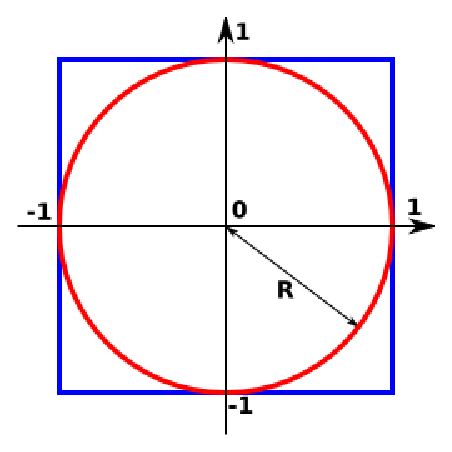
\includegraphics[width=0.4\textwidth]{montecarlopi}
    \caption{计算圆周率$\pi$}\label{fig:pi2}
    \vspace{\baselineskip}
    \end{figure}

现在我们在正方形内部挑选任意$N$个点,挑选任意点这个动作属于随机动作(当随机点产生的越多,其结果越接近于圆周率),接下来检查此点是否被包含在
圆内,如果符合$x^2+y^2 < R^2$则认为是在圆内部,同时记录属于圆内部的点数量$M$,如图~\ref{fig:pi3},红色点表示在圆内的点,红色点的数量
等于$N-M$,黑色点表示不属于圆的点,数目为$M$,此时$\pi$约等于
    \[ \pi \simeq \frac{4*M}{N} \]
    
    \begin{figure}[htbp]
    \centering
    
\includegraphics[width=0.4\textwidth]{square}
    \caption{挑选随机点$\pi$}\label{fig:pi3}
    \vspace{\baselineskip}
    \end{figure}

\section{并行算法}
        
    蒙特卡罗算法求解园周率$\pi$的计算方法,由于各个随机数产生的行为和判断行为都是并行的,可以分解为多个任务相同的子问题,
各个子间相互独立,易实现良好的并行性,在这里使用MPI将任务进行划分,将每个子问题分解到不同的计算结点上,各个计算结点计
算结果后主结点进行汇总求和,最终得到求得的$\pi$值。整个并行算法流程有server进程用来产生随机数队列,master主进程用来请请求和管理
随机队列,并且分配任务给worker进程,worker进程负责计算和返回计算结果并且请求随机数队列,算法如图~\ref{fig:pisqe}:
    \begin{figure}[ht]
    \centering
    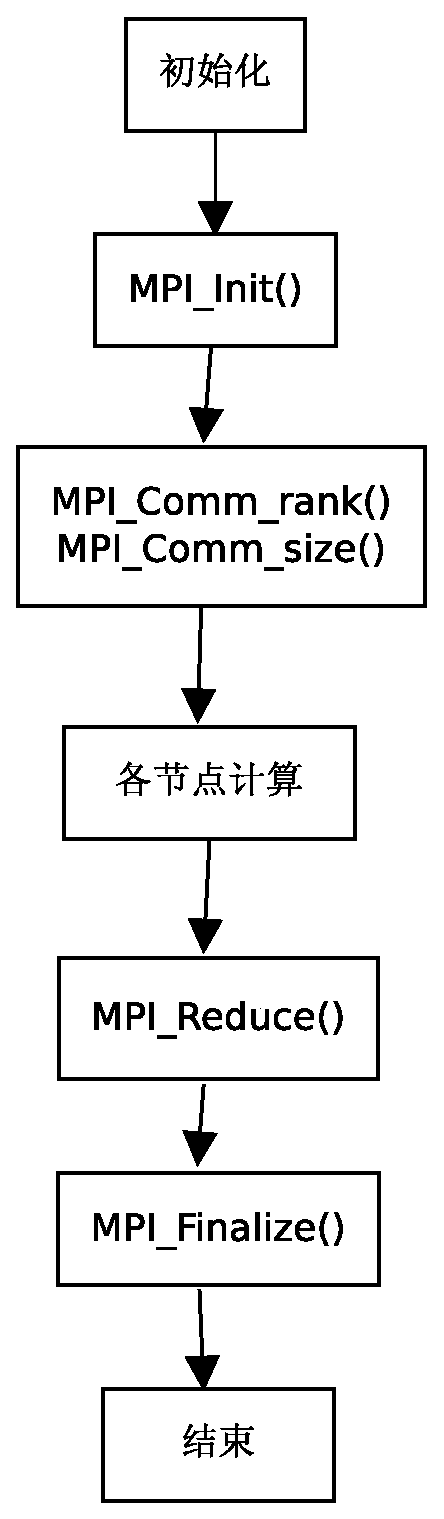
\includegraphics[width=1.0\textwidth]{pisqe}
    \caption{并行化计算$\pi$}\label{fig:pisqe}
    \vspace{\baselineskip}
    \end{figure}


\section{算法伪代码}
    以下部分为算法的伪代码
\algrenewcommand{\algorithmiccomment}[1]{\hskip3em$\rightarrow$ #1}
\begin{algorithmic}[1]
\State $actualpi  \gets 3.141592653589793238462643$
\Comment 初始化真实的$\pi$,对比计算所得的$\pi$
\State $calcpi,temppi,sum,\ldots$
\Comment 初始化需要用到的变量值
\State $MPI::Init()$
\State $world = MPI\_COMM\_WORLD$
\State $ MPI\_Comm\_size(world,numprocs)$
\State $ MPI\_Comm\_rank(world,myid)$
\Comment 初始化PMI
\If {$ master $}
    \State $MPI\_Bcast{dotsnumber}$
    \State $MPI\_Comm\_create(world,worker\_group,workers)$
\EndIf
\If {$ Server $}
    \State $MPI\_Recv(request)$
    \State $Generate random numbers array$
    \State $MPI\_Send(random numers array)$
\Else
    \State $MPI\_Send(send request to server)$
    \While{$!Done$}
            \State $MPI\_Recv(Server sumdata)$
        \For {$i \gets 0 to N-1 $}
            \State  $ x=rand(i) and  y = rand(i) $ 
            \If{$ x*x + y*y < 1.0$} 
                \State $M+1$
            \EndIf
        \EndFor
        \State $MPI\_Allreduce(in)$
        \State $MPI\_Allreduce(out)$

        \State $pi=(4.0*totalin)/(in+out)$

        \If {$master$}
                \State  $ print \pi$
                \Comment 输出结算所得的$\pi$
        \EndIf    
        \If{$worker$} 
            \If {$request$}
                \State $MPI\_Send(server,request)$
            \EndIf 
        \EndIf 
    \EndWhile
\EndIf

\If {$主进程$}
    \State $输出结果$
    \State $MPI\_Finalize()$
\EndIf
\end{algorithmic}

\section{实验结果}
\subsection{加速比}
    传统算法的时间复杂度为$O(N)$,并行算法的时间复杂度为$O(\frac{N}{p})$,所以并行化的加速比为
    $$S=\frac{O(N)}{O(\frac{N}{p})}$$

\subsection{实验结果分析}
本次试验结果通过MPI内置的的MPI\_Wtime()来统计程序的运行时间,分别采用单机和并行化的方式来统计程序运行的时间和效率,
每次程序的运行时间通过多次实验采取平均值的方法,下表是计算时间随计算结点数目的不同而变化的试验结果图


\begin{tikzpicture}
\begin{loglogaxis}[
height=10cm,
width=10cm,
xlabel=点的数量,
ylabel=估计时间,
ymin=0,
xmin=0,
legend style ={
    area legend,
    at ={(0.5,-0.15)},
    anchor = north,
    legend columns = -1}
]

\addplot coordinates {
(1,0)
(10001,3e-03)
(20050,5e-03)
(30060,7.5e-03)
(40200,1e-02)
(50700,1.25e-02)
(60900,1.5e-02)
(70000,1.75e-02)
(80080,2e-02)
(90070,2.5e-02)
};

\addplot coordinates {
(1,0)
(10001,2e-03)
(20050,3e-03)
(30060,5.5e-03)
(40200,7e-03)
(50700,1.0e-02)
(60900,1.2e-02)
(70000,1.35e-02)
(80080,1.7e-02)
(90070,2.0e-02)
};
\addplot coordinates {
(1,0)
(10001,2e-03)
(20050,3e-03)
(30060,4.5e-03)
(40200,6e-03)
(50700,0.8e-02)
(60900,1.0e-02)
(70000,1.2e-02)
(80080,1.4e-02)
(90070,1.6e-02)
};

\legend{Np=01,Np=02,Np=03}
\end{loglogaxis}
\end{tikzpicture}

通过此图可以看出并行计算和单机计算相比来说,时间效率更高,单位时间内计算量更大。

当计算节点数目不多时,MPI的算法呈直线增长,但是当节点数目增加时,由于进程间通信消耗时间增多,导致增长
速度缓慢,而单机串行算法始终保持一种线性关系的增长。


接下来是4核机器的测试时间展示

%\begin{table}[htbp]
%\centering  % 表居中
%\begin{tabular}{lcc}  % {lccc} 表示各列元素对齐方式,left-l,right-r,center-c
%\hline
%Step &非并行算法时间&并行算法时间 \\ \hline  % \hline 在此行下面画一横线
%1000&0.001 &0.00014 \\        
%10000&0.002 &0.00016 \\      
%100000&0.004 &0.00053 \\     
%1000000&0.026&0.0081 \\   
%10000000&0.187&0.05\\
%100000000&1.838 & 0.463\\
%1000000000&18.325& 5.46368\\ 
%10000000000&15:38.325&7.878 \\ \hline
%\end{tabular}
%\caption{算法时间对比总结}
%\end{table}

%http://www.angio.net/pi/pi-programs.html
%http://www.cnblogs.com/zhangchaoyang/articles/1871168.html
